\documentclass[tikz,border=8pt]{standalone}
% Shared look for every TikZ diagram. Load with \input{../../tools/tikz-style.tex}
\usepackage[sfdefault]{roboto}
\usetikzlibrary{arrows.meta, positioning, shapes.geometric, calc, fit, backgrounds}
\definecolor{cblue}{HTML}{4C78A8}
\definecolor{corange}{HTML}{F58518}
\definecolor{cgreen}{HTML}{54A24B}
\definecolor{cred}{HTML}{E45756}
\definecolor{cpurple}{HTML}{B279A2}
\definecolor{cgrey}{HTML}{6B6B6B}
\tikzset{
  every picture/.style={font=\sffamily, line width=1.2pt},
  box/.style={draw=#1, fill=#1!12, rounded corners=4pt, align=center, inner sep=7pt, minimum height=1.1cm},
  box/.default=cgrey,
  arrow/.style={-{Stealth[length=3mm]}, draw=cgrey, line width=1.4pt},
  title/.style={font=\sffamily\bfseries\Large},
  note/.style={font=\sffamily\small, text=cgrey, align=center},
}
\AtBeginDocument{\hyphenpenalty=10000 \exhyphenpenalty=10000}

% PDDL: the domain file (predicates and actions, written once) and the problem file (objects, start state, goal)
% go into a planner, which returns the plan. A second problem file reuses the same domain file.
\begin{document}
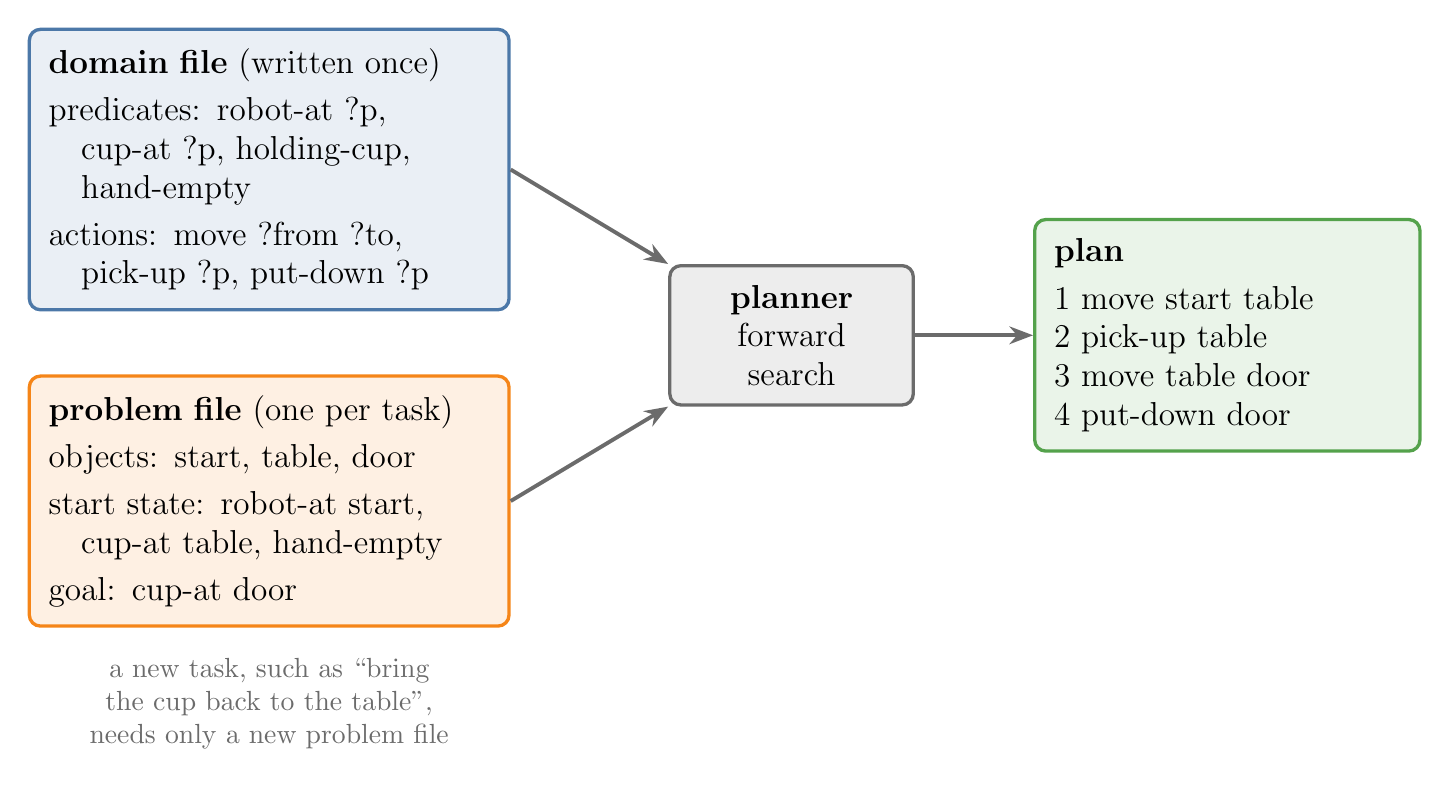
\begin{tikzpicture}[every node/.append style={font=\large}, node distance=1.2cm]
  \node[box=cblue, text width=5.6cm, align=left] (d) {\textbf{domain file} (written once)\\[3pt]
    predicates: robot-at ?p,\\ \quad cup-at ?p, holding-cup,\\ \quad hand-empty\\[3pt]
    actions: move ?from ?to,\\ \quad pick-up ?p, put-down ?p};
  \node[box=corange, text width=5.6cm, align=left, below=0.8cm of d] (p) {\textbf{problem file} (one per task)\\[3pt]
    objects: start, table, door\\[3pt]
    start state: robot-at start,\\ \quad cup-at table, hand-empty\\[3pt]
    goal: cup-at door};
  \node[box=cgrey, right=2.0cm of $(d.east)!0.5!(p.east)$, minimum height=1.6cm, text width=2.6cm, align=center]
    (pl) {\textbf{planner}\\ forward search};
  \node[box=cgreen, right=1.5cm of pl, text width=4.4cm, align=left] (o) {\textbf{plan}\\[3pt]
    1 move start table\\ 2 pick-up table\\ 3 move table door\\ 4 put-down door};
  \draw[arrow] (d.east) -- (pl.north west);
  \draw[arrow] (p.east) -- (pl.south west);
  \draw[arrow] (pl) -- (o);
  \node[note, below=0.25cm of p, text width=5.6cm, font=\normalsize] {a new task, such as ``bring the cup back to the table'', needs only a new problem file};
\end{tikzpicture}
\end{document}
